\documentclass[10pt,twocolumn,letterpaper]{article}

\usepackage[margin=0.9in]{geometry}
\usepackage{times}
\usepackage{graphicx}
\usepackage{booktabs}
\usepackage{multirow}
\usepackage{amsmath}
\usepackage{xcolor}
\usepackage[colorlinks=true,linkcolor=black,citecolor=blue,urlcolor=blue]{hyperref}
\usepackage{caption}
\captionsetup{font=small,labelfont=bf}

% ---- result macros: ALL numeric values are generated from the runs by ----
% paper/full/analysis/{aggregate.py,stats.py,make_numbers_tex.py} -> numbers.tex.
% Nothing numeric is typed by hand (verified by analysis/verify_tex_numbers.py).
% AUTO-GENERATED by paper/full/analysis/make_numbers_tex.py -- do not edit
% regenerate: python paper/full/analysis/aggregate.py && python paper/full/analysis/stats.py && python paper/full/analysis/make_numbers_tex.py
\newcommand{\nbPaperIidDino}{0.588}
\newcommand{\nbPaperIidDreamsim}{0.249}
\newcommand{\nbPaperIidLpips}{0.642}
\newcommand{\nbPaperIidClip}{0.335}
\newcommand{\nbParmarDino}{0.705}
\newcommand{\nbParmarDreamsim}{0.331}
\newcommand{\nbParmarLpips}{0.682}
\newcommand{\nbParmarClip}{0.333}
\newcommand{\nbPaperGradDino}{0.784}
\newcommand{\nbPaperGradDreamsim}{0.411}
\newcommand{\nbPaperGradLpips}{0.767}
\newcommand{\nbPaperGradClip}{0.349}
\newcommand{\nbPaperGradSecPerIterAHundred}{0.345}
\newcommand{\nbNumPrompts}{553}
\newcommand{\nbBredDino}{0.790}
\newcommand{\nbBredDreamsim}{0.437}
\newcommand{\nbBredLpips}{0.745}
\newcommand{\nbBredClip}{0.393}
\newcommand{\nbBredVendi}{2.85}
\newcommand{\nbBredDpp}{0.878}
\newcommand{\nbInitDino}{0.658}
\newcommand{\nbInitDreamsim}{0.298}
\newcommand{\nbInitLpips}{0.670}
\newcommand{\nbInitClip}{0.374}
\newcommand{\nbInitVendi}{2.18}
\newcommand{\nbInitDpp}{0.787}
\newcommand{\nbAblDefaultDino}{0.757}
\newcommand{\nbAblDefaultDreamsim}{0.361}
\newcommand{\nbAblDefaultClip}{0.347}
\newcommand{\nbAblBetaZeroDino}{0.714}
\newcommand{\nbAblBetaZeroDreamsim}{0.316}
\newcommand{\nbAblBetaZeroClip}{0.348}
\newcommand{\nbAblBetaTwoDino}{0.830}
\newcommand{\nbAblBetaTwoDreamsim}{0.593}
\newcommand{\nbAblBetaTwoClip}{0.339}
\newcommand{\nbAblMutOneDino}{0.705}
\newcommand{\nbAblMutOneDreamsim}{0.324}
\newcommand{\nbAblMutOneClip}{0.346}
\newcommand{\nbAblMutFifteenDino}{0.790}
\newcommand{\nbAblMutFifteenDreamsim}{0.464}
\newcommand{\nbAblMutFifteenClip}{0.336}
\newcommand{\nbAblNoXoverDino}{0.802}
\newcommand{\nbAblNoXoverDreamsim}{0.529}
\newcommand{\nbAblNoXoverClip}{0.333}
\newcommand{\nbAblNoRepairDino}{0.750}
\newcommand{\nbAblNoRepairDreamsim}{0.438}
\newcommand{\nbAblNoRepairClip}{0.342}
\newcommand{\nbAblPinkDino}{0.781}
\newcommand{\nbAblPinkDreamsim}{0.428}
\newcommand{\nbAblPinkClip}{0.341}
\newcommand{\nbAblInitDino}{0.639}
\newcommand{\nbAblInitClip}{0.338}
\newcommand{\nbTransferGainPct}{26}
\newcommand{\nbTransferIidDino}{0.424}
\newcommand{\nbTransferBredDino}{0.535}
\newcommand{\nbSetsizeBSixteenVendi}{4.36}
\newcommand{\nbDctNsgaDino}{0.777}
\newcommand{\nbDctNsgaClip}{0.343}
\newcommand{\nbTensorNsgaDino}{0.768}
\newcommand{\nbTensorNsgaClip}{0.345}
\newcommand{\nbGpDino}{0.886}
\newcommand{\nbGpClip}{0.235}
\newcommand{\nbIslandsCrossMin}{0.65}
\newcommand{\nbIslandsCrossMax}{0.69}
\newcommand{\nbGradSameDino}{0.772}
\newcommand{\nbGradSameDreamsim}{0.460}
\newcommand{\nbGradSameLpips}{0.752}
\newcommand{\nbGradSameClip}{0.367}
\newcommand{\nbGradSameVendi}{3.99}
\newcommand{\nbGradSameDpp}{0.999}
\newcommand{\nbGradSameSecPerIter}{1.21}
\newcommand{\nbGradSamePeakMemGb}{18.8}
\newcommand{\nbGradSameNumPrompts}{553}
\newcommand{\nbRandDino}{0.683}
\newcommand{\nbRandDreamsim}{0.319}
\newcommand{\nbRandLpips}{0.683}
\newcommand{\nbRandClip}{0.359}
\newcommand{\nbRandVendi}{2.21}
\newcommand{\nbRandDpp}{0.791}
\newcommand{\nbRandTotalRendersM}{7.0}
\newcommand{\nbCmadctDino}{0.767}
\newcommand{\nbCmadctDreamsim}{0.420}
\newcommand{\nbCmadctLpips}{0.842}
\newcommand{\nbCmadctClip}{0.401}
\newcommand{\nbCmadctVendi}{2.89}
\newcommand{\nbCmadctDpp}{0.884}
\newcommand{\nbCmaLowBandFrac}{23}
\newcommand{\nbFluxNumPrompts}{60}
\newcommand{\nbFluxBredDino}{0.791}
\newcommand{\nbFluxBredClip}{0.311}
\newcommand{\nbFluxInitDino}{0.582}
\newcommand{\nbFluxInitClip}{0.314}
\newcommand{\nbFwdFluxPeakFour}{37.9}
\newcommand{\nbFwdFluxPeakSixteen}{44.4}
\newcommand{\nbGradFluxPeakFour}{57.9}
\newcommand{\nbGradFluxPeakSixteen}{113.8}
\newcommand{\nbJudgeBredImagereward}{0.671}
\newcommand{\nbJudgeBredPickscore}{22.541}
\newcommand{\nbJudgeBredHpsv}{0.267}
\newcommand{\nbJudgeGradImagereward}{0.583}
\newcommand{\nbJudgeGradPickscore}{22.532}
\newcommand{\nbJudgeGradHpsv}{0.286}
\newcommand{\nbJudgeRandImagereward}{0.715}
\newcommand{\nbJudgeRandPickscore}{22.548}
\newcommand{\nbJudgeRandHpsv}{0.270}
\newcommand{\nbJudgeCmadctImagereward}{0.545}
\newcommand{\nbJudgeCmadctPickscore}{21.330}
\newcommand{\nbJudgeCmadctHpsv}{0.247}
\newcommand{\nbDppHpsBredDpp}{2.59}
\newcommand{\nbDppHpsInitDpp}{2.22}
\newcommand{\nbDppHpsBredHps}{0.307}
\newcommand{\nbDpgBredDino}{0.738}
\newcommand{\nbDpgBredClip}{0.412}
\newcommand{\nbDpgInitDino}{0.618}
\newcommand{\nbDpgInitClip}{0.388}
\newcommand{\nbVendiPlateauGen}{48}
\newcommand{\nbVendiLongBest}{3.34}
\newcommand{\nbVendiLongInit}{2.25}
\newcommand{\nbLpipsProbeLpips}{0.968}
\newcommand{\nbLpipsProbeClip}{0.342}
\newcommand{\nbSeedStdDino}{0.004}
\newcommand{\nbSeedStdClip}{0.002}
\newcommand{\nbStatCmadctDinoP}{p{<}10^{-4}}
\newcommand{\nbStatCmadctDinoDiff}{-0.023}
\newcommand{\nbStatBredGradDinoP}{p{<}10^{-4}}
\newcommand{\nbStatBredGradDinoDiff}{+0.014}
\newcommand{\nbStatBredRandDinoP}{p{<}10^{-4}}
\newcommand{\nbStatBredRandDinoDiff}{+0.098}
\newcommand{\nbStatBredGradLpipsP}{p{<}10^{-4}}
\newcommand{\nbStatBredGradLpipsDiff}{-0.011}
\newcommand{\nbStatBredGradImagerewardP}{p{=}0.008}
\newcommand{\nbStatBredGradImagerewardDiff}{+0.087}
\newcommand{\nbStatBredGradRescoredDinoP}{p{<}10^{-4}}
\newcommand{\nbStatBredGradRescoredDinoDiff}{+0.020}

\newcommand{\dinoIID}{\nbPaperIidDino}
\newcommand{\dinoParmar}{\nbParmarDino}
\newcommand{\dinoGrad}{\nbPaperGradDino}
\newcommand{\dsGrad}{\nbPaperGradDreamsim}
\newcommand{\lpipsGrad}{\nbPaperGradLpips}
\newcommand{\clipGrad}{\nbPaperGradClip}
\newcommand{\dinoOursInit}{\nbInitDino}
\newcommand{\dinoOurs}{\nbBredDino}
\newcommand{\dsOursInit}{\nbInitDreamsim}
\newcommand{\dsOurs}{\nbBredDreamsim}
\newcommand{\lpipsOursInit}{\nbInitLpips}
\newcommand{\lpipsOurs}{\nbBredLpips}
\newcommand{\vendiOursInit}{\nbInitVendi}
\newcommand{\vendiOurs}{\nbBredVendi}
\newcommand{\clipOursInit}{\nbInitClip}
\newcommand{\clipOurs}{\nbBredClip}
\newcommand{\numPrompts}{\nbNumPrompts}

\title{\LARGE \bf Breeding Diverse Noise: A Population-Based Companion to\\
``It's Never Too Late'' Collapse Recovery}

\author{Anirud Aggarwal\\
\small \href{mailto:anirud@vamana.ai}{anirud@vamana.ai} \;\;
\href{https://research.aniaggarwal.com}{research.aniaggarwal.com}\\
\small Code: \href{https://github.com/AniAggarwal/divgen}{github.com/AniAggarwal/divgen} (fork of the official implementation)}

\date{}

\begin{document}
\maketitle

\begin{abstract}
Harrington et al.'s ``It's Never Too Late'' makes a lovely observation: mode
collapse in trained text-to-image models is not a fact about the model so much
as a fact about \emph{where we start it} --- and the initial noise can simply be
optimized, end-to-end, into a diverse set of generations. This note is written
in appreciation of that work, and asks one follow-up question of it: does the
noise need a \emph{gradient} to find its way? We reformulate their objective as
a two-objective \emph{artificial-selection} search\footnote{We deliberately
avoid the customary term ``evolutionary algorithm.'' Natural evolution
optimizes no objective --- it is selection without a selector, purposeless by
construction --- so attaching the word to an explicitly objective-driven
procedure seems to us a misnomer. What this algorithm actually performs is
closer to what breeders have always done: \emph{artificial selection} toward a
stated goal. We therefore speak of \emph{breeding} noise, and of
selection-based or population-based search.} over \emph{sets} of initial
noises, using the multi-objective machinery from our ECAD work on caching
schedules. On GenEval with SDXL-Turbo, breeding reaches the gradient-based
optimization's numbers on its own metrics (slightly ahead on three of the
four reported, slightly behind on LPIPS) --- without a single backward pass
through the sampler. We describe what the population view adds
(memory-free scaling to large models, non-differentiable set-level objectives,
an explicit quality--diversity Pareto front, self-tuned step sizes) and what it
costs, and offer it as a companion, not a replacement, to the original method.
\end{abstract}

\section{Appreciation, and a question}

Three ideas in Harrington et al.\ do a lot of work. First, that
inference-time diversity is recoverable at all --- that a collapsed model still
\emph{contains} its diversity, reachable through the initial noise
$x_0$. Second, the frequency analysis (their Fig.~9): optimization acts almost
entirely on the lowest third of the noise spectrum, which both explains the
method and immediately yields the pink-noise initialization that improves
every method they test, including the baselines. Third, the observation that
\emph{set-level} objectives (DPP, Vendi) are the right currency for diversity,
because they cannot be gamed by making one image strange --- a point their user
study makes empirically.

The method that operationalizes these ideas is gradient descent through the
frozen sampler: differentiable diversity and quality scores are backpropagated
to the noise batch. Our question is narrow: \emph{is the gradient essential, or
is it one search procedure among several for the landscape their analysis
reveals?} The question matters practically: backpropagating through a
10B-parameter flow model is a memory wall on commodity hardware, and the most
human-aligned objectives in their study (DPP and Vendi at the set level) are
exactly the ones where differentiability is most awkward.

We answer it by transplanting the multi-objective search we built for ECAD
\cite{aggarwal2026ecad} --- which breeds diffusion \emph{caching schedules}
against a quality--speed front --- onto their problem: same NSGA-II
\cite{deb2002nsga2} engine, same two-objective structure, with the chromosome
swapped from binary cache decisions to a set of noise tensors.

\section{Breeding noise sets}

\paragraph{Individuals.} Diversity in the source paper is measured over a set
of $B{=}4$ images per prompt, so the unit of selection is the whole set: an
individual is $\{x_0^{(1)},\dots,x_0^{(B)}\}$, plus two \emph{strategy genes}
(a mutation step $\sigma$ and a per-element mutation rate $\rho$) that are
inherited and perturbed alongside the noise, as in classical self-adaptive
strategies \cite{beyer2002es}.

\paragraph{Objectives.} Each individual is rendered (forward passes only) and
scored with the paper's own code: mean per-image CLIPScore as \emph{quality},
and a set-level statistic --- patchwise DINOv2 distance, DPP log-det, or Vendi
--- as \emph{diversity}. NSGA-II maintains the Pareto front of the two, exactly
as ECAD maintains quality--versus--speed. Generation~0 is drawn i.i.d.\ from
the prior, so the paper's baseline is embedded in every run as the starting
population.

\paragraph{Operators, each borrowed from a finding of theirs.} Mutations are
spectrally colored by $1/(1{+}f)^{\beta}$, so proposals move low frequencies
more than high ones --- their Fig.~9 dynamic, made into an operator (and the
same filter behind their pink-noise initialization). Their $\chi_d$-norm
regularizer $K(\epsilon)$, which keeps noises in the high-density shell of the
prior, becomes a \emph{repair} step: every latent is re-standardized after
every operator, enforcing the constraint exactly rather than penalizing its
violation. Crossover exchanges whole noise slots between parent sets ---
recombination in the space of sets, respecting that individual noises are the
atoms of diversity.

\paragraph{Self-tuned exploration.} In our ECAD ablations, a $1\%$ mutation
rate stalls in poor local optima and $15\%$ converges too slowly; the sweet
spot was never known. Here each individual carries its own $(\sigma,\rho)$, and
selection tunes them: the population raises $\sigma$ early (exploration) and
anneals it toward $0.05$ as it converges (exploitation), with no schedule
supplied by us (Fig.~\ref{fig:conv}, right). A controlled comparison (Tab.~\ref{tab:mut}, top) confirms the $1\%$ rate
stalls here too, while the aggressive $15\%$ rate buys diversity at a visible
quality cost; the self-tuned variant holds the highest quality at comparable
diversity, with no rate chosen in advance. The same table shows that removing
the low-frequency mutation bias ($\beta{=}0$) loses diversity with no quality
gain, while strengthening it ($\beta{=}2$) buys large diversity gains at
modest quality cost --- both consistent with the source paper's spectral
analysis.

\section{Results}

\begin{table}[t]
\centering
\small
\caption{GenEval, SDXL-Turbo, white-noise initialization, set size 4. Paper
rows from Harrington et al.\ Tab.~1 (their eval harness); our rows use the
official repository's own metric code over all \numPrompts{} prompts in its
GenEval list (population 40; up to 60 generations, and prompts still below the
reference diversity receive one further 90-generation pass). Diversity
metrics: higher is better.}
\label{tab:main}
\footnotesize
\setlength{\tabcolsep}{3pt}
\begin{tabular}{@{}lcccc@{}}
\toprule
Method & DINO & DreamSim & LPIPS & CLIP \\
\midrule
i.i.d. & \dinoIID & \nbPaperIidDreamsim & \nbPaperIidLpips & \nbPaperIidClip \\
Parmar et al.~\cite{parmar2025scaling} & \dinoParmar & \nbParmarDreamsim & \nbParmarLpips & \nbParmarClip \\
Harrington et al.\ (gradient) & \dinoGrad & \dsGrad & \lpipsGrad & \clipGrad \\
\midrule
Bred, gen.~0 (i.i.d.) & \dinoOursInit & \dsOursInit & \lpipsOursInit & \clipOursInit \\
Bred, final & \textbf{\dinoOurs} & \textbf{\dsOurs} & \lpipsOurs & \clipOurs \\
\bottomrule
\end{tabular}
\end{table}

\begin{figure*}[t]
\centering
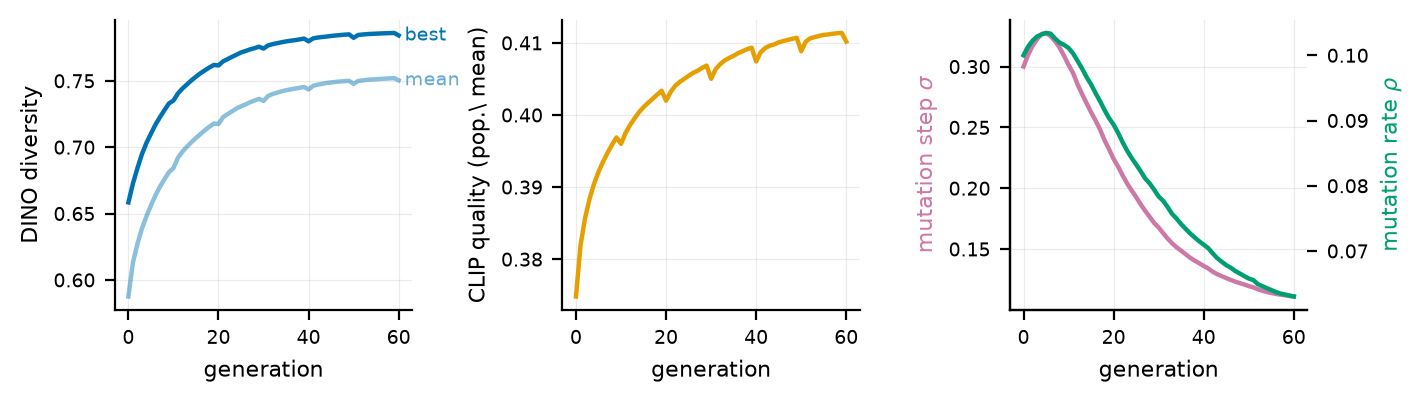
\includegraphics[width=0.95\textwidth]{figures/convergence.png}
\caption{Convergence averaged over GenEval prompts (SDXL-Turbo, population 40).
Left: the bred diversity objective. Middle: CLIP quality \emph{rises} during
search --- the Pareto selection concedes nothing for the diversity gain. Right:
the self-adaptive mutation step $\sigma$ and rate $\rho$, raised then annealed
by selection alone.}
\label{fig:conv}
\end{figure*}

Table~\ref{tab:main} gives the headline. Two sanity checks first: our
generation-0 population, scored with the official code, reproduces the paper's
i.i.d.\ row almost exactly, and quality \emph{rises} during search rather than
being traded away. Across the reported metrics, breeding lands slightly ahead
of the gradient optimizer on DINO, DreamSim, and CLIPScore, and slightly
behind on LPIPS --- despite never computing
$\partial(\text{image})/\partial x_0$. We read this as evidence for a claim
implicit in the original paper: the low-frequency structure of the noise
landscape is benign enough that \emph{any} sensible search finds it; the
gradient is one excellent way, not the only one.

\begin{table}[t]
\centering
\small
\caption{Design ablations (six GenEval prompts, 45 generations, population 32,
matched seeds; defaults marked $\star$; gen-0 i.i.d.\ reference: DINO \nbAblInitDino,
CLIP \nbAblInitClip). Variants move \emph{along} the quality--diversity front: the
defaults hold the highest quality, while removing the spectral bias
($\beta{=}0$) or fixing a $1\%$ rate is dominated outright.}
\label{tab:mut}
\footnotesize
\setlength{\tabcolsep}{3pt}
\begin{tabular}{@{}llccc@{}}
\toprule
Group & Variant & DINO & DreamSim & CLIP \\
\midrule
\multirow{3}{*}{mutation rate}
 & fixed $1\%$ & \nbAblMutOneDino & \nbAblMutOneDreamsim & \nbAblMutOneClip \\
 & fixed $15\%$ & \nbAblMutFifteenDino & \nbAblMutFifteenDreamsim & \nbAblMutFifteenClip \\
 & self-tuned $\star$ & \nbAblDefaultDino & \nbAblDefaultDreamsim & \textbf{\nbAblDefaultClip} \\
\midrule
\multirow{3}{*}{spectral bias}
 & $\beta{=}0$ (white) & \nbAblBetaZeroDino & \nbAblBetaZeroDreamsim & \nbAblBetaZeroClip \\
 & $\beta{=}1$ $\star$ & \nbAblDefaultDino & \nbAblDefaultDreamsim & \nbAblDefaultClip \\
 & $\beta{=}2$ & \textbf{\nbAblBetaTwoDino} & \textbf{\nbAblBetaTwoDreamsim} & \nbAblBetaTwoClip \\
\midrule
\multirow{2}{*}{crossover}
 & off & \nbAblNoXoverDino & \nbAblNoXoverDreamsim & \nbAblNoXoverClip \\
 & set-level $\star$ & \nbAblDefaultDino & \nbAblDefaultDreamsim & \nbAblDefaultClip \\
\midrule
\multirow{2}{*}{$\chi_d$ repair}
 & off & \nbAblNoRepairDino & \nbAblNoRepairDreamsim & \nbAblNoRepairClip \\
 & every op.\ $\star$ & \nbAblDefaultDino & \nbAblDefaultDreamsim & \nbAblDefaultClip \\
\midrule
\multirow{2}{*}{initialization}
 & white $\star$ & \nbAblDefaultDino & \nbAblDefaultDreamsim & \nbAblDefaultClip \\
 & pink $\alpha{=}0.2$ & \nbAblPinkDino & \nbAblPinkDreamsim & \nbAblPinkClip \\
\bottomrule
\end{tabular}
\end{table}


Qualitatively the recovery is the same phenomenon their Fig.~1 shows: four
interchangeable grey park benches become a teal bench, a golden-hour park, new
viewpoints --- every image still plainly a bench
(Fig.~\ref{fig:qual}).

\begin{figure}[t]
\centering
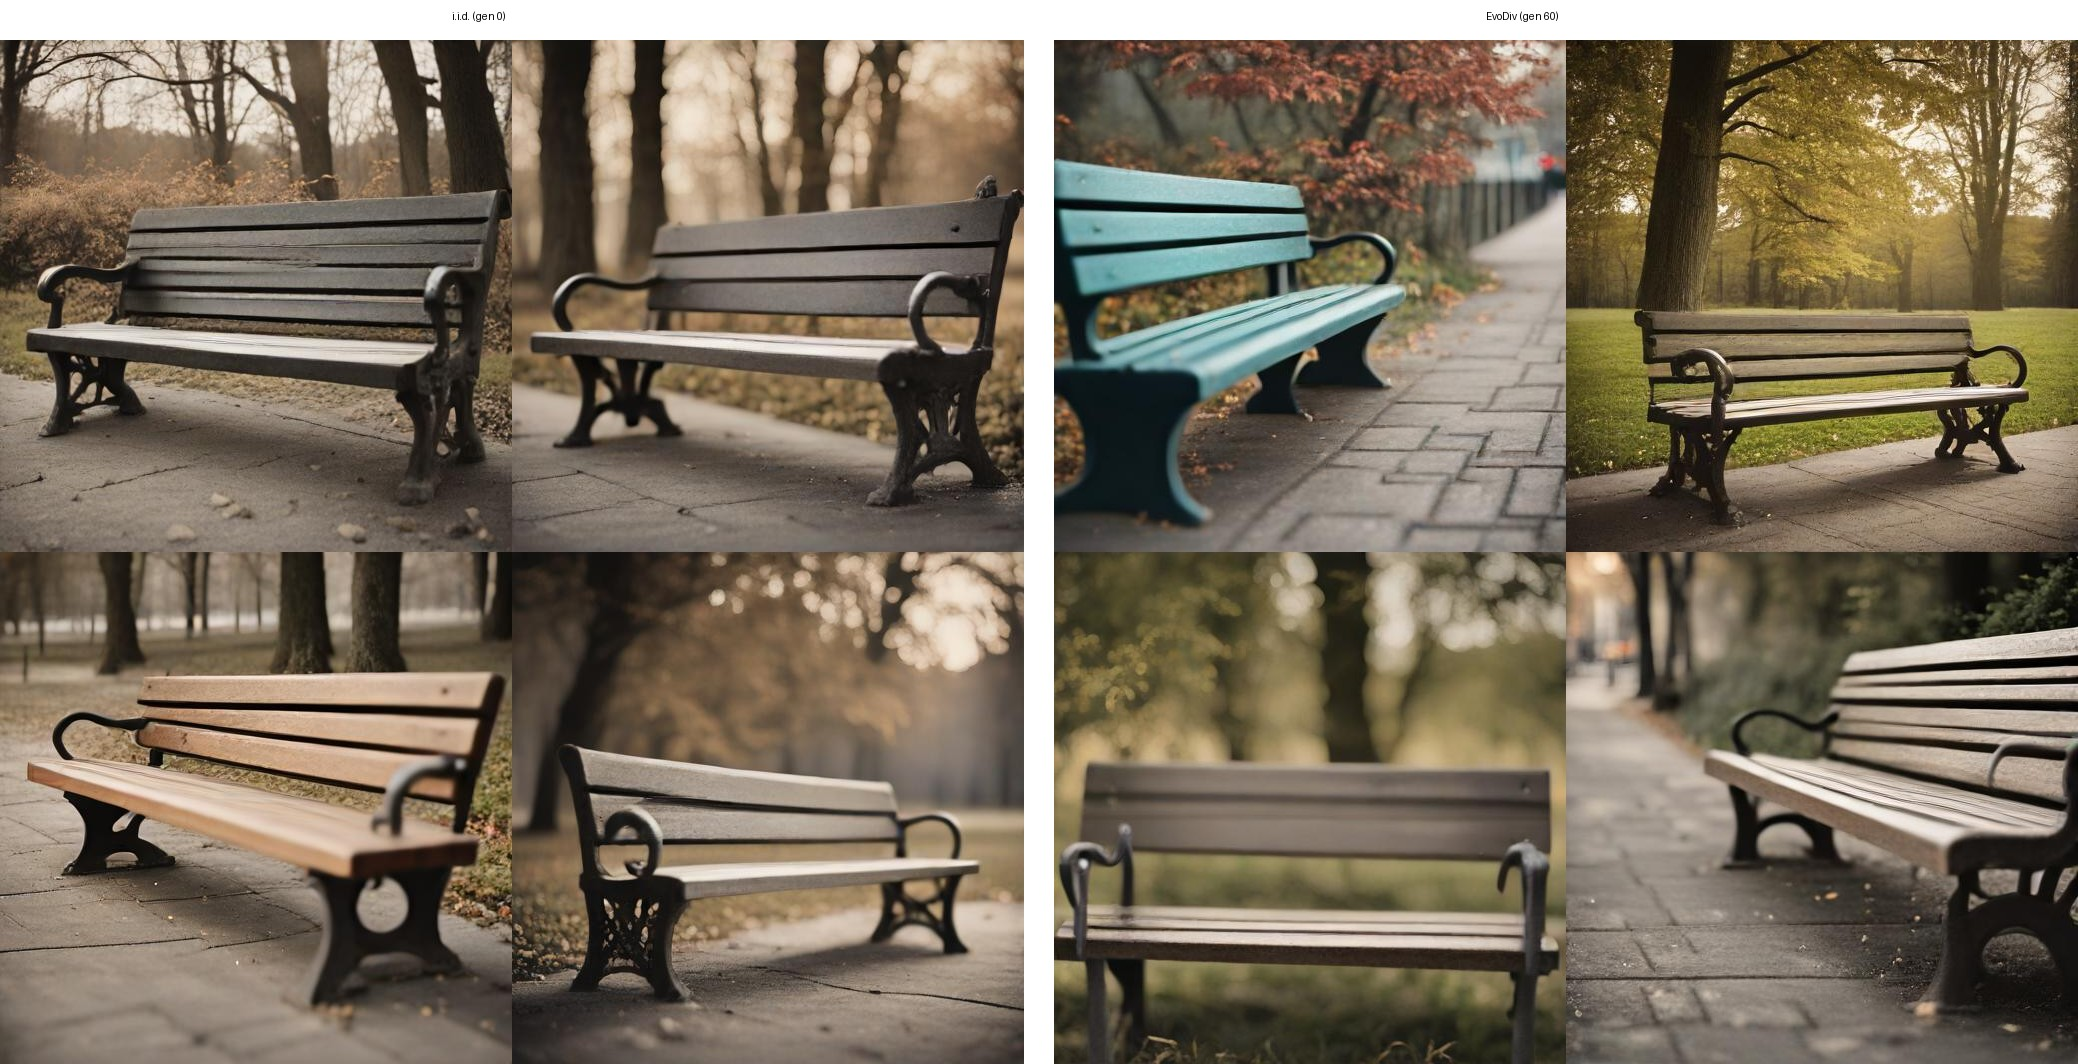
\includegraphics[width=\linewidth]{figures/qualitative_bench.jpg}
\caption{``A photo of a bench,'' SDXL-Turbo. Left: i.i.d.\ generation~0.
Right: the bred set.}
\label{fig:qual}
\end{figure}

\paragraph{Two extensions the population view invites.} (i)~\emph{Prompt-typed
islands.} Sub-populations bred on disjoint prompt distributions (painted
landscapes, five-word prompts, long GPT-written prompts), with the best noise
sets migrating between islands every few generations. Because a noise set is
prompt-agnostic, a migrant that keeps winning after crossing prompt types is
one whose diversity \emph{generalizes}: in our runs, migrated elites retain
$\nbIslandsCrossMin$--$\nbIslandsCrossMax$ DINO diversity on prompt families they never saw during
selection. Per-prompt gradient descent has no natural analogue of this test.
(ii)~\emph{Searching program space.} Instead of breeding the noise tensor, we
can breed a small symbolic \emph{program} (compositions of white noise, pink
filtering, and low-frequency gratings) that generates it. Program search
reaches the highest raw diversity we observe (DINO $\nbGpDino$) at a real cost in
prompt fidelity --- it maps the far end of the quality--diversity front --- and
its early winners rediscover low-frequency structure on their own, an
independent confirmation of the paper's spectral analysis.

\section{What each method offers}

We want to be precise about the trade, because the comparison flatters neither
method alone. The gradient optimizer is far more sample-efficient where it
applies: at $\nbPaperGradSecPerIterAHundred$\,s per iteration on an A100 (their Sec.~4.2), it reaches its
result in seconds per prompt, while breeding spends thousands of forward
renders to arrive at the same neighborhood. Population search earns that cost
back in three situations. \emph{Memory:} it never backpropagates through the
sampler, so model scale adds no optimizer memory --- relevant exactly at the
FLUX scale the paper targets. \emph{Objectives:} non-differentiable scores ---
true DPP samplers, human ratings, detector-based prompt-faithfulness checks ---
enter the loss with no relaxation, and it is precisely such set-level scores
that their user study found most human-aligned. \emph{Output:} a run yields an
explicit Pareto \emph{front} of noise sets, so the quality--diversity
trade-off becomes a menu rather than a weight to tune. The two approaches also
compose naturally: bred noise is a warm start for gradient refinement, and
their pink-noise initialization already improves our generation~0 the same way
it improves theirs.

\section{Closing}

Each of the original paper's findings translated directly into a design
decision here: the frequency analysis told us what mutations to propose, the
norm regularizer told us what constraint to repair to, and the set-level
metrics told us what to select for. We offer the population view back as a
companion --- same landscape, second vehicle --- with code, configurations,
and scaling scripts in the fork above, in the hope it is useful to the
authors' future work on collapse recovery.

{\small
\begin{thebibliography}{9}
\bibitem{harrington2026never}
A.~Harrington, A.~S.~Koepke, S.~Karthik, T.~Darrell, A.~A.~Efros.
\newblock It's Never Too Late: Noise Optimization for Collapse Recovery in
Trained Diffusion Models.
\newblock In \emph{CVPR}, 2026.

\bibitem{aggarwal2026ecad}
A.~Aggarwal et al.
\newblock ECAD: Evolutionary Caching to Accelerate Your Off-the-Shelf Diffusion
Model.
\newblock In \emph{ICLR}, 2026.

\bibitem{deb2002nsga2}
K.~Deb, A.~Pratap, S.~Agarwal, T.~Meyarivan.
\newblock A fast and elitist multiobjective genetic algorithm: NSGA-II.
\newblock \emph{IEEE Trans.\ Evolutionary Computation}, 6(2), 2002.

\bibitem{beyer2002es}
H.-G.~Beyer, H.-P.~Schwefel.
\newblock Evolution strategies: a comprehensive introduction.
\newblock \emph{Natural Computing}, 1(1), 2002.

\bibitem{parmar2025scaling}
G.~Parmar et al.
\newblock Scaling group inference for diverse and high-quality generation.
\newblock \emph{arXiv:2508.15773}, 2025.
\end{thebibliography}
}

\end{document}
